% Options for packages loaded elsewhere
\PassOptionsToPackage{unicode}{hyperref}
\PassOptionsToPackage{hyphens}{url}
%
\documentclass[
]{article}
\usepackage{amsmath,amssymb}
\usepackage{lmodern}
\usepackage{ifxetex,ifluatex}
\ifnum 0\ifxetex 1\fi\ifluatex 1\fi=0 % if pdftex
  \usepackage[T1]{fontenc}
  \usepackage[utf8]{inputenc}
  \usepackage{textcomp} % provide euro and other symbols
\else % if luatex or xetex
  \usepackage{unicode-math}
  \defaultfontfeatures{Scale=MatchLowercase}
  \defaultfontfeatures[\rmfamily]{Ligatures=TeX,Scale=1}
\fi
% Use upquote if available, for straight quotes in verbatim environments
\IfFileExists{upquote.sty}{\usepackage{upquote}}{}
\IfFileExists{microtype.sty}{% use microtype if available
  \usepackage[]{microtype}
  \UseMicrotypeSet[protrusion]{basicmath} % disable protrusion for tt fonts
}{}
\makeatletter
\@ifundefined{KOMAClassName}{% if non-KOMA class
  \IfFileExists{parskip.sty}{%
    \usepackage{parskip}
  }{% else
    \setlength{\parindent}{0pt}
    \setlength{\parskip}{6pt plus 2pt minus 1pt}}
}{% if KOMA class
  \KOMAoptions{parskip=half}}
\makeatother
\usepackage{xcolor}
\IfFileExists{xurl.sty}{\usepackage{xurl}}{} % add URL line breaks if available
\IfFileExists{bookmark.sty}{\usepackage{bookmark}}{\usepackage{hyperref}}
\hypersetup{
  pdftitle={Introduction to R},
  hidelinks,
  pdfcreator={LaTeX via pandoc}}
\urlstyle{same} % disable monospaced font for URLs
\usepackage[margin=1in]{geometry}
\usepackage{color}
\usepackage{fancyvrb}
\newcommand{\VerbBar}{|}
\newcommand{\VERB}{\Verb[commandchars=\\\{\}]}
\DefineVerbatimEnvironment{Highlighting}{Verbatim}{commandchars=\\\{\}}
% Add ',fontsize=\small' for more characters per line
\usepackage{framed}
\definecolor{shadecolor}{RGB}{248,248,248}
\newenvironment{Shaded}{\begin{snugshade}}{\end{snugshade}}
\newcommand{\AlertTok}[1]{\textcolor[rgb]{0.94,0.16,0.16}{#1}}
\newcommand{\AnnotationTok}[1]{\textcolor[rgb]{0.56,0.35,0.01}{\textbf{\textit{#1}}}}
\newcommand{\AttributeTok}[1]{\textcolor[rgb]{0.77,0.63,0.00}{#1}}
\newcommand{\BaseNTok}[1]{\textcolor[rgb]{0.00,0.00,0.81}{#1}}
\newcommand{\BuiltInTok}[1]{#1}
\newcommand{\CharTok}[1]{\textcolor[rgb]{0.31,0.60,0.02}{#1}}
\newcommand{\CommentTok}[1]{\textcolor[rgb]{0.56,0.35,0.01}{\textit{#1}}}
\newcommand{\CommentVarTok}[1]{\textcolor[rgb]{0.56,0.35,0.01}{\textbf{\textit{#1}}}}
\newcommand{\ConstantTok}[1]{\textcolor[rgb]{0.00,0.00,0.00}{#1}}
\newcommand{\ControlFlowTok}[1]{\textcolor[rgb]{0.13,0.29,0.53}{\textbf{#1}}}
\newcommand{\DataTypeTok}[1]{\textcolor[rgb]{0.13,0.29,0.53}{#1}}
\newcommand{\DecValTok}[1]{\textcolor[rgb]{0.00,0.00,0.81}{#1}}
\newcommand{\DocumentationTok}[1]{\textcolor[rgb]{0.56,0.35,0.01}{\textbf{\textit{#1}}}}
\newcommand{\ErrorTok}[1]{\textcolor[rgb]{0.64,0.00,0.00}{\textbf{#1}}}
\newcommand{\ExtensionTok}[1]{#1}
\newcommand{\FloatTok}[1]{\textcolor[rgb]{0.00,0.00,0.81}{#1}}
\newcommand{\FunctionTok}[1]{\textcolor[rgb]{0.00,0.00,0.00}{#1}}
\newcommand{\ImportTok}[1]{#1}
\newcommand{\InformationTok}[1]{\textcolor[rgb]{0.56,0.35,0.01}{\textbf{\textit{#1}}}}
\newcommand{\KeywordTok}[1]{\textcolor[rgb]{0.13,0.29,0.53}{\textbf{#1}}}
\newcommand{\NormalTok}[1]{#1}
\newcommand{\OperatorTok}[1]{\textcolor[rgb]{0.81,0.36,0.00}{\textbf{#1}}}
\newcommand{\OtherTok}[1]{\textcolor[rgb]{0.56,0.35,0.01}{#1}}
\newcommand{\PreprocessorTok}[1]{\textcolor[rgb]{0.56,0.35,0.01}{\textit{#1}}}
\newcommand{\RegionMarkerTok}[1]{#1}
\newcommand{\SpecialCharTok}[1]{\textcolor[rgb]{0.00,0.00,0.00}{#1}}
\newcommand{\SpecialStringTok}[1]{\textcolor[rgb]{0.31,0.60,0.02}{#1}}
\newcommand{\StringTok}[1]{\textcolor[rgb]{0.31,0.60,0.02}{#1}}
\newcommand{\VariableTok}[1]{\textcolor[rgb]{0.00,0.00,0.00}{#1}}
\newcommand{\VerbatimStringTok}[1]{\textcolor[rgb]{0.31,0.60,0.02}{#1}}
\newcommand{\WarningTok}[1]{\textcolor[rgb]{0.56,0.35,0.01}{\textbf{\textit{#1}}}}
\usepackage{longtable,booktabs,array}
\usepackage{calc} % for calculating minipage widths
% Correct order of tables after \paragraph or \subparagraph
\usepackage{etoolbox}
\makeatletter
\patchcmd\longtable{\par}{\if@noskipsec\mbox{}\fi\par}{}{}
\makeatother
% Allow footnotes in longtable head/foot
\IfFileExists{footnotehyper.sty}{\usepackage{footnotehyper}}{\usepackage{footnote}}
\makesavenoteenv{longtable}
\usepackage{graphicx}
\makeatletter
\def\maxwidth{\ifdim\Gin@nat@width>\linewidth\linewidth\else\Gin@nat@width\fi}
\def\maxheight{\ifdim\Gin@nat@height>\textheight\textheight\else\Gin@nat@height\fi}
\makeatother
% Scale images if necessary, so that they will not overflow the page
% margins by default, and it is still possible to overwrite the defaults
% using explicit options in \includegraphics[width, height, ...]{}
\setkeys{Gin}{width=\maxwidth,height=\maxheight,keepaspectratio}
% Set default figure placement to htbp
\makeatletter
\def\fps@figure{htbp}
\makeatother
\setlength{\emergencystretch}{3em} % prevent overfull lines
\providecommand{\tightlist}{%
  \setlength{\itemsep}{0pt}\setlength{\parskip}{0pt}}
\setcounter{secnumdepth}{5}
\ifluatex
  \usepackage{selnolig}  % disable illegal ligatures
\fi

\title{Introduction to R}
\author{}
\date{\vspace{-2.5em}}

\usepackage{amsthm}
\newtheorem{theorem}{Theorem}[section]
\newtheorem{lemma}{Lemma}[section]
\newtheorem{corollary}{Corollary}[section]
\newtheorem{proposition}{Proposition}[section]
\newtheorem{conjecture}{Conjecture}[section]
\theoremstyle{definition}
\newtheorem{definition}{Definition}[section]
\theoremstyle{definition}
\newtheorem{example}{Example}[section]
\theoremstyle{definition}
\newtheorem{exercise}{Exercise}[section]
\theoremstyle{remark}
\newtheorem*{remark}{Remark}
\newtheorem*{solution}{Solution}
\begin{document}
\maketitle

{
\setcounter{tocdepth}{2}
\tableofcontents
}
\hypertarget{what-is-r}{%
\section{What is R?}\label{what-is-r}}

R is a free open-source program that is used to do statistics in both academia and industry. There are many online resources for R, for both beginners and experts. For example, \href{https://cran.r-project.org/doc/manuals/r-release/R-intro.pdf}{Venables, Smith, and the R Core Team}

\hypertarget{a-fancy-calculator}{%
\subsection{A fancy calculator}\label{a-fancy-calculator}}

R can be used as a fancy calculator

\begin{Shaded}
\begin{Highlighting}[]
\DecValTok{2}\SpecialCharTok{+}\DecValTok{2}
\end{Highlighting}
\end{Shaded}

\begin{verbatim}
## [1] 4
\end{verbatim}

\begin{Shaded}
\begin{Highlighting}[]
\FunctionTok{sin}\NormalTok{(}\FloatTok{3.14}\NormalTok{)}
\end{Highlighting}
\end{Shaded}

\begin{verbatim}
## [1] 0.001592653
\end{verbatim}

\begin{Shaded}
\begin{Highlighting}[]
\FunctionTok{exp}\NormalTok{(}\DecValTok{1}\NormalTok{)}
\end{Highlighting}
\end{Shaded}

\begin{verbatim}
## [1] 2.718282
\end{verbatim}

\begin{Shaded}
\begin{Highlighting}[]
\FunctionTok{log}\NormalTok{(}\FloatTok{2.71}\NormalTok{)}
\end{Highlighting}
\end{Shaded}

\begin{verbatim}
## [1] 0.9969486
\end{verbatim}

\begin{Shaded}
\begin{Highlighting}[]
\NormalTok{pi}
\end{Highlighting}
\end{Shaded}

\begin{verbatim}
## [1] 3.141593
\end{verbatim}

Variables can be assigned in the following way

\begin{Shaded}
\begin{Highlighting}[]
\NormalTok{x }\OtherTok{\textless{}{-}} \DecValTok{1}\SpecialCharTok{+}\DecValTok{2}\SpecialCharTok{+}\DecValTok{3}\SpecialCharTok{+}\DecValTok{4}\SpecialCharTok{+}\DecValTok{5}\SpecialCharTok{+}\DecValTok{6}
\NormalTok{x}\SpecialCharTok{*}\DecValTok{2}
\end{Highlighting}
\end{Shaded}

\begin{verbatim}
## [1] 42
\end{verbatim}

\hypertarget{entering-data-by-hand-into-r}{%
\subsection{Entering data by hand into R}\label{entering-data-by-hand-into-r}}

R is designed to store data as vectors \(x = (x_1, x_2, \ldots, x_n)\) that is lists of numbers.

\begin{Shaded}
\begin{Highlighting}[]
\NormalTok{y }\OtherTok{\textless{}{-}} \FunctionTok{c}\NormalTok{(}\DecValTok{1}\NormalTok{,}\DecValTok{2}\NormalTok{,}\DecValTok{3}\NormalTok{,}\DecValTok{4}\NormalTok{,}\DecValTok{5}\NormalTok{,}\DecValTok{6}\NormalTok{,}\DecValTok{7}\NormalTok{,}\DecValTok{8}\NormalTok{,}\DecValTok{9}\NormalTok{)}
\NormalTok{y}
\end{Highlighting}
\end{Shaded}

\begin{verbatim}
## [1] 1 2 3 4 5 6 7 8 9
\end{verbatim}

\hypertarget{basic-operations-with-vectors}{%
\subsection{Basic operations with vectors}\label{basic-operations-with-vectors}}

R has many built in common operations that are useful for statistics:

\begin{Shaded}
\begin{Highlighting}[]
\NormalTok{x }\OtherTok{\textless{}{-}} \FunctionTok{c}\NormalTok{(}\DecValTok{1}\NormalTok{,}\DecValTok{2}\NormalTok{,}\DecValTok{3}\NormalTok{,}\DecValTok{4}\NormalTok{,}\DecValTok{5}\NormalTok{,}\DecValTok{6}\NormalTok{,}\DecValTok{7}\NormalTok{,}\DecValTok{8}\NormalTok{,}\DecValTok{9}\NormalTok{,}\DecValTok{10}\NormalTok{)}
\NormalTok{x}
\end{Highlighting}
\end{Shaded}

\begin{verbatim}
##  [1]  1  2  3  4  5  6  7  8  9 10
\end{verbatim}

\begin{Shaded}
\begin{Highlighting}[]
\FunctionTok{sum}\NormalTok{(x)}
\end{Highlighting}
\end{Shaded}

\begin{verbatim}
## [1] 55
\end{verbatim}

\begin{Shaded}
\begin{Highlighting}[]
\FunctionTok{mean}\NormalTok{(x)}
\end{Highlighting}
\end{Shaded}

\begin{verbatim}
## [1] 5.5
\end{verbatim}

\begin{Shaded}
\begin{Highlighting}[]
\FunctionTok{sd}\NormalTok{(x)}
\end{Highlighting}
\end{Shaded}

\begin{verbatim}
## [1] 3.02765
\end{verbatim}

\begin{Shaded}
\begin{Highlighting}[]
\FunctionTok{var}\NormalTok{(x)}
\end{Highlighting}
\end{Shaded}

\begin{verbatim}
## [1] 9.166667
\end{verbatim}

R will do certain operations component wise:

\begin{Shaded}
\begin{Highlighting}[]
\NormalTok{ x }\OtherTok{\textless{}{-}} \FunctionTok{c}\NormalTok{(}\DecValTok{1}\NormalTok{,}\DecValTok{2}\NormalTok{,}\DecValTok{3}\NormalTok{,}\DecValTok{4}\NormalTok{,}\DecValTok{5}\NormalTok{)}
\NormalTok{y }\OtherTok{\textless{}{-}} \FunctionTok{c}\NormalTok{(}\DecValTok{6}\NormalTok{,}\DecValTok{7}\NormalTok{,}\DecValTok{8}\NormalTok{,}\DecValTok{9}\NormalTok{,}\DecValTok{10}\NormalTok{)}
\NormalTok{z}\OtherTok{=}\NormalTok{x}\SpecialCharTok{+}\NormalTok{y}
\NormalTok{z}
\end{Highlighting}
\end{Shaded}

\begin{verbatim}
## [1]  7  9 11 13 15
\end{verbatim}

\begin{Shaded}
\begin{Highlighting}[]
\NormalTok{x}\SpecialCharTok{*}\NormalTok{y}
\end{Highlighting}
\end{Shaded}

\begin{verbatim}
## [1]  6 14 24 36 50
\end{verbatim}

\begin{Shaded}
\begin{Highlighting}[]
\FunctionTok{sin}\NormalTok{(z)}
\end{Highlighting}
\end{Shaded}

\begin{verbatim}
## [1]  0.6569866  0.4121185 -0.9999902  0.4201670  0.6502878
\end{verbatim}

It is often necessary to add or delete data from a vector:

\begin{Shaded}
\begin{Highlighting}[]
\NormalTok{x}\OtherTok{\textless{}{-}} \FunctionTok{c}\NormalTok{(}\FloatTok{0.1}\NormalTok{, }\FloatTok{0.2}\NormalTok{, }\FloatTok{0.3}\NormalTok{, }\FloatTok{0.4}\NormalTok{, }\FloatTok{0.5}\NormalTok{)}
\NormalTok{x }\OtherTok{\textless{}{-}}\NormalTok{ x[}\SpecialCharTok{{-}}\DecValTok{5}\NormalTok{]}
\NormalTok{x}
\end{Highlighting}
\end{Shaded}

\begin{verbatim}
## [1] 0.1 0.2 0.3 0.4
\end{verbatim}

\begin{Shaded}
\begin{Highlighting}[]
\NormalTok{x }\OtherTok{\textless{}{-}} \FunctionTok{c}\NormalTok{(x, }\FloatTok{5.5}\NormalTok{)}
\NormalTok{x}
\end{Highlighting}
\end{Shaded}

\begin{verbatim}
## [1] 0.1 0.2 0.3 0.4 5.5
\end{verbatim}

\hypertarget{coin-flips-dice-roll-normal-and-uniform-random-variables-in-r}{%
\subsection{Coin-flips, dice roll, normal, and uniform random variables in R}\label{coin-flips-dice-roll-normal-and-uniform-random-variables-in-r}}

R can be used to simulate coin flips and dice roll. R does not use true randomness, rather it generates coin clips using a deterministic algorithm that simulates true randomness.

\begin{Shaded}
\begin{Highlighting}[]
\NormalTok{x}\OtherTok{\textless{}{-}} \FunctionTok{rbinom}\NormalTok{(}\DecValTok{12}\NormalTok{,}\DecValTok{1}\NormalTok{, }\FloatTok{0.5}\NormalTok{)}
\NormalTok{x}
\end{Highlighting}
\end{Shaded}

\begin{verbatim}
##  [1] 1 1 0 1 0 1 1 0 1 0 0 1
\end{verbatim}

\begin{Shaded}
\begin{Highlighting}[]
\NormalTok{z }\OtherTok{\textless{}{-}} \FunctionTok{sample}\NormalTok{(}\DecValTok{6}\NormalTok{,}\DecValTok{12}\NormalTok{, }\AttributeTok{replace =}\ConstantTok{TRUE}\NormalTok{)}
\NormalTok{z}
\end{Highlighting}
\end{Shaded}

\begin{verbatim}
##  [1] 6 3 6 6 6 4 3 5 1 1 1 1
\end{verbatim}

\begin{Shaded}
\begin{Highlighting}[]
\NormalTok{x}\OtherTok{\textless{}{-}} \FunctionTok{rnorm}\NormalTok{(}\DecValTok{10}\NormalTok{, }\DecValTok{5}\NormalTok{, }\DecValTok{1}\NormalTok{)}
\NormalTok{x}
\end{Highlighting}
\end{Shaded}

\begin{verbatim}
##  [1] 4.364105 5.607793 5.611612 5.465956 5.615734 4.342180 4.358493 4.370943
##  [9] 5.538732 3.992501
\end{verbatim}

\begin{Shaded}
\begin{Highlighting}[]
\NormalTok{z }\OtherTok{\textless{}{-}} \FunctionTok{runif}\NormalTok{(}\DecValTok{10}\NormalTok{, }\AttributeTok{min=}\SpecialCharTok{{-}}\DecValTok{1}\NormalTok{, }\AttributeTok{max=}\DecValTok{1}\NormalTok{)}
\NormalTok{z}
\end{Highlighting}
\end{Shaded}

\begin{verbatim}
##  [1] -0.51791536 -0.63960814 -0.35067838 -0.83028156 -0.23804930  0.71187486
##  [7] -0.89146324 -0.04485452  0.82136771 -0.11007441
\end{verbatim}

\hypertarget{histograms-in-r}{%
\section{Histograms in R}\label{histograms-in-r}}

\begin{Shaded}
\begin{Highlighting}[]
\NormalTok{x }\OtherTok{\textless{}{-}} \FunctionTok{rexp}\NormalTok{(}\DecValTok{100}\NormalTok{,}\DecValTok{1}\NormalTok{)}
\FunctionTok{hist}\NormalTok{(x, }\AttributeTok{prob=}\ConstantTok{TRUE}\NormalTok{)}
\end{Highlighting}
\end{Shaded}

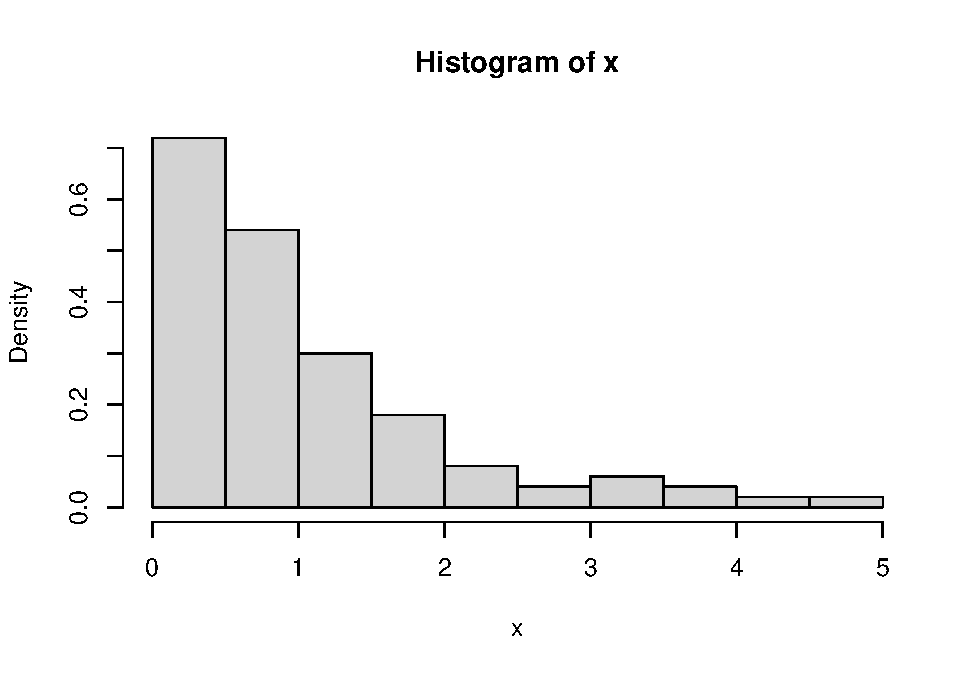
\includegraphics{intro-R_files/figure-latex/unnamed-chunk-8-1.pdf}
Here \(x\) is a 100 randomly generated data points from the exponential distribution with rate \(1\).

\hypertarget{functions}{%
\section{Functions}\label{functions}}

Suppose we needed to use the quantity \(\sin(x) + \cos(x)\) over and over again for different values of \(x\), then it may be useful to define this as a function in the following way:

\begin{Shaded}
\begin{Highlighting}[]
\NormalTok{sincos }\OtherTok{\textless{}{-}} \ControlFlowTok{function}\NormalTok{(x)\{}
\NormalTok{z }\OtherTok{\textless{}{-}} \FunctionTok{sin}\NormalTok{(x) }\SpecialCharTok{+} \FunctionTok{cos}\NormalTok{(x);}
\NormalTok{z}
\NormalTok{\}}
\FunctionTok{sincos}\NormalTok{(}\DecValTok{1}\NormalTok{)}
\end{Highlighting}
\end{Shaded}

\begin{verbatim}
## [1] 1.381773
\end{verbatim}

Here the function sincos takes an input \(x\). It is sometimes useful have functions that do not take inputs, but simple perform operations: say roll a fair dice 1o times, and take the sum.

\hypertarget{basic-programming-in-r}{%
\section{Basic programming in R}\label{basic-programming-in-r}}

We will introduce basic programming in R with the following exercise and will illustrate how to write a \emph{while} loop in R.
\begin{exercise}
\protect\hypertarget{exr:unnamed-chunk-10}{}{\label{exr:unnamed-chunk-10} }By running simulations in R, approximate the average number of rolls of a fair dice it takes before you see a 6.
\end{exercise}
\begin{solution}
\iffalse{} {Solution. } \fi{}We make a function \emph{numrolls} which counts how many times we need to roll a dice until we see a \(6\). Then we use the \emph{replicate} command to repeat this function many time, and take the average.
\end{solution}

\begin{Shaded}
\begin{Highlighting}[]
\NormalTok{numrolls }\OtherTok{\textless{}{-}} \ControlFlowTok{function}\NormalTok{()\{}
\NormalTok{n}\OtherTok{=}\DecValTok{0}
\NormalTok{x}\OtherTok{=}\DecValTok{0}
\ControlFlowTok{while}\NormalTok{(x }\SpecialCharTok{\textless{}}\DecValTok{6}\NormalTok{)\{}
\NormalTok{x }\OtherTok{\textless{}{-}} \FunctionTok{sample}\NormalTok{(}\DecValTok{6}\NormalTok{,}\DecValTok{1}\NormalTok{, }\AttributeTok{replace =}\ConstantTok{TRUE}\NormalTok{)}
\NormalTok{n }\OtherTok{\textless{}{-}}\NormalTok{ n}\SpecialCharTok{+}\DecValTok{1}
\NormalTok{\}}
\NormalTok{n}
\NormalTok{\}}

\FunctionTok{mean}\NormalTok{(}\FunctionTok{replicate}\NormalTok{(}\DecValTok{1000}\NormalTok{, }\FunctionTok{numrolls}\NormalTok{()) )}
\end{Highlighting}
\end{Shaded}

\begin{verbatim}
## [1] 5.866
\end{verbatim}

In the next exercise, we illustrate how to write a \emph{for} loop.

\begin{exercise}
\protect\hypertarget{exr:unnamed-chunk-13}{}{\label{exr:unnamed-chunk-13} }Define a function that tells you whether a positive integer is prime or not.
\end{exercise}
\begin{solution}
\iffalse{} {Solution. } \fi{}Let \(n\) be an integer. We first recall that \(d\) is a divisor of \(n\) if there exists an integer \(c\) such that \$ n = cd\$. An integer \(n \geq 2\) is prime if it only divisors are \(1\) and \(n\). R has a built in remainder function, which for nonnegative integers \(a,b\) outputs the remainder in the sense of elementary school, when \(a\) is divided by \(b\). Using the remainder function we define the \emph{isprime} function, and use it spit out the prime numbers up to 500.
\end{solution}

\begin{Shaded}
\begin{Highlighting}[]
\DecValTok{25}\SpecialCharTok{\%\%}\DecValTok{5}
\end{Highlighting}
\end{Shaded}

\begin{verbatim}
## [1] 0
\end{verbatim}

\begin{Shaded}
\begin{Highlighting}[]
\DecValTok{26}\SpecialCharTok{\%\%}\DecValTok{5}
\end{Highlighting}
\end{Shaded}

\begin{verbatim}
## [1] 1
\end{verbatim}

\begin{Shaded}
\begin{Highlighting}[]
\NormalTok{isprime }\OtherTok{\textless{}{-}} \ControlFlowTok{function}\NormalTok{(n)\{}
\NormalTok{x}\OtherTok{=}\DecValTok{1}
\ControlFlowTok{for}\NormalTok{ (i }\ControlFlowTok{in} \DecValTok{2}\SpecialCharTok{:}\NormalTok{ (n}\DecValTok{{-}1}\NormalTok{))\{}
\ControlFlowTok{if}\NormalTok{ (x }\SpecialCharTok{\textgreater{}}\DecValTok{0}\NormalTok{) \{}
\NormalTok{x }\OtherTok{\textless{}{-}}\NormalTok{ n}\SpecialCharTok{\%\%}\NormalTok{i}
\NormalTok{\}}
\NormalTok{\}}
\ControlFlowTok{if}\NormalTok{ (n}\SpecialCharTok{==}\DecValTok{1}\NormalTok{) \{x }\OtherTok{\textless{}{-}}\DecValTok{0}\NormalTok{\}}
\ControlFlowTok{if}\NormalTok{ (n}\SpecialCharTok{==}\DecValTok{2}\NormalTok{) \{x }\OtherTok{\textless{}{-}}\DecValTok{1}\NormalTok{\}}
\NormalTok{ x}
\NormalTok{ \}}
 \FunctionTok{isprime}\NormalTok{(}\DecValTok{1}\NormalTok{)}
\end{Highlighting}
\end{Shaded}

\begin{verbatim}
## [1] 0
\end{verbatim}

\begin{Shaded}
\begin{Highlighting}[]
 \FunctionTok{isprime}\NormalTok{(}\DecValTok{2}\NormalTok{)}
\end{Highlighting}
\end{Shaded}

\begin{verbatim}
## [1] 1
\end{verbatim}

\begin{Shaded}
\begin{Highlighting}[]
\FunctionTok{isprime}\NormalTok{(}\DecValTok{101}\NormalTok{)}
\end{Highlighting}
\end{Shaded}

\begin{verbatim}
## [1] 1
\end{verbatim}

\begin{Shaded}
\begin{Highlighting}[]
\NormalTok{x}\OtherTok{=}\DecValTok{2}
 \ControlFlowTok{for}\NormalTok{(i }\ControlFlowTok{in} \DecValTok{3}\SpecialCharTok{:}\DecValTok{500}\NormalTok{)\{}
\ControlFlowTok{if}\NormalTok{( }\FunctionTok{isprime}\NormalTok{(i)}\SpecialCharTok{==}\DecValTok{1}\NormalTok{)\{}
\NormalTok{x }\OtherTok{\textless{}{-}} \FunctionTok{c}\NormalTok{(x, i)\}}
\NormalTok{ x}
\NormalTok{\}}
\NormalTok{x}
\end{Highlighting}
\end{Shaded}

\begin{verbatim}
##  [1]   2   3   5   7  11  13  17  19  23  29  31  37  41  43  47  53  59  61  67
## [20]  71  73  79  83  89  97 101 103 107 109 113 127 131 137 139 149 151 157 163
## [39] 167 173 179 181 191 193 197 199 211 223 227 229 233 239 241 251 257 263 269
## [58] 271 277 281 283 293 307 311 313 317 331 337 347 349 353 359 367 373 379 383
## [77] 389 397 401 409 419 421 431 433 439 443 449 457 461 463 467 479 487 491 499
\end{verbatim}

\hypertarget{summary}{%
\section{Summary}\label{summary}}

We introduced some basics of R, and we gave examples programming basics including defining functions, while loops, for loops, and using the replicate function.

\hypertarget{version-25-september-2020}{%
\section{Version: 25 September 2020}\label{version-25-september-2020}}

\end{document}
